\chapter{Astronomical data} \label{chap:astronomicaldata}

% nejaky obkec o tom ze data sa ziskavaju cez teleskopy a tie maju CCD chipy a ze snimky su vo formate FITS. a potom ze v tejto casti prejdeme rozne features ktore sa na snimkach nachadzaju, scenare a defekty a ako tieto nezaduce data odstranujeme
% FITS frames
% AGO data

In this section, we will first talk about how space debris images are acquired. We will describe the parameters of the telescope that captured the images used within this thesis. We will also define the format of the astronomical images. Next, we will explain what type of features can be present on the images and the defects and noises affecting them. In the last section, we present the image calibration process that is used to reduce the noises and defects to achieve clean images used for further processing and analysis. 

\section{AGO70}
The space debris images are acquired using astronomical telescopes. 
In our thesis, we are working with images captured at the Astronomical and Geophysical Observatory (AGO) in Modra. The acquisition of images at AGO is performed by the reflecting Newtonian telescope (AGO70) \cite{ago702018}, shown in the Figure \ref{img:ago70}. 

\begin{figure}[h]
    \centering
    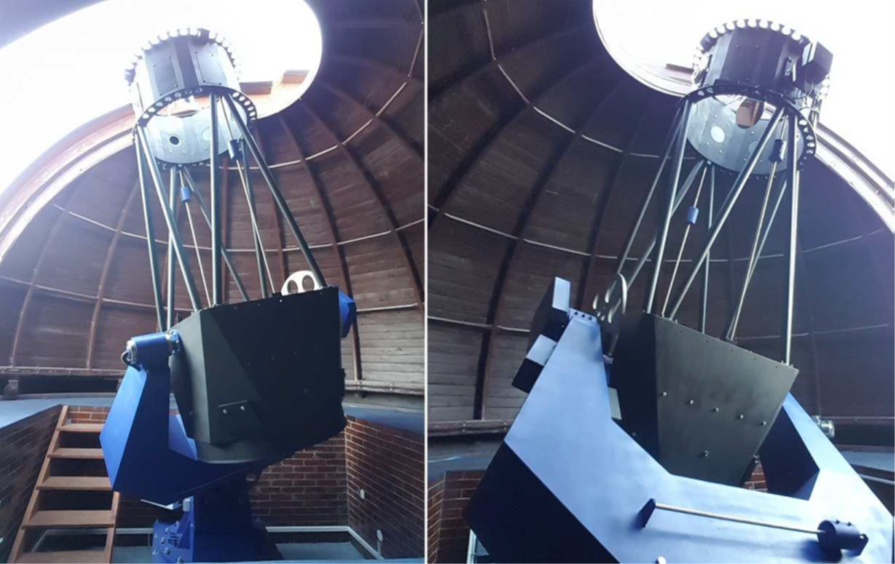
\includegraphics[width=.5\textwidth]{images/ago70.png}
    \caption{The telescope AGO70 in Modra. Source: \cite{ago702018}.}
    \label{img:ago70}
\end{figure}

In 2016, after Slovakia became the 9th member of the ESA Plan for the European Cooperating States (PECS), a contract with the Faculty of Mathematics, Physics, and Informatics (FMPI) was signed. The first action was to transform the telescope in AGO from an amateur observation tool into a professional optical system used for regular tracking of space debris. Some examples of images acquired from the space debris observations performed by AGO70 are shown in the Figure \ref{fig:ago70images}. The installation of AGO70 finished in 2016 and the telescope has the following parameters: 

\begin{itemize}
    \item 700 mm primary parabolic mirror
    \item gravity actuator supporting the parabolic mirror
    \item focal length of 2962 mm
    \item FLI Proline PL1001 Grade 1 CCD camera
    \item 24 $\mu$m pixel size of the CCD camera
    \item resolution 1024x1024
    \item 28.5' x 28.5' field of view
    \item 16 bit per pixel images
\end{itemize}


\begin{figure}[!h]
    \begin{subfigure}{.3\textwidth}
        \centering
        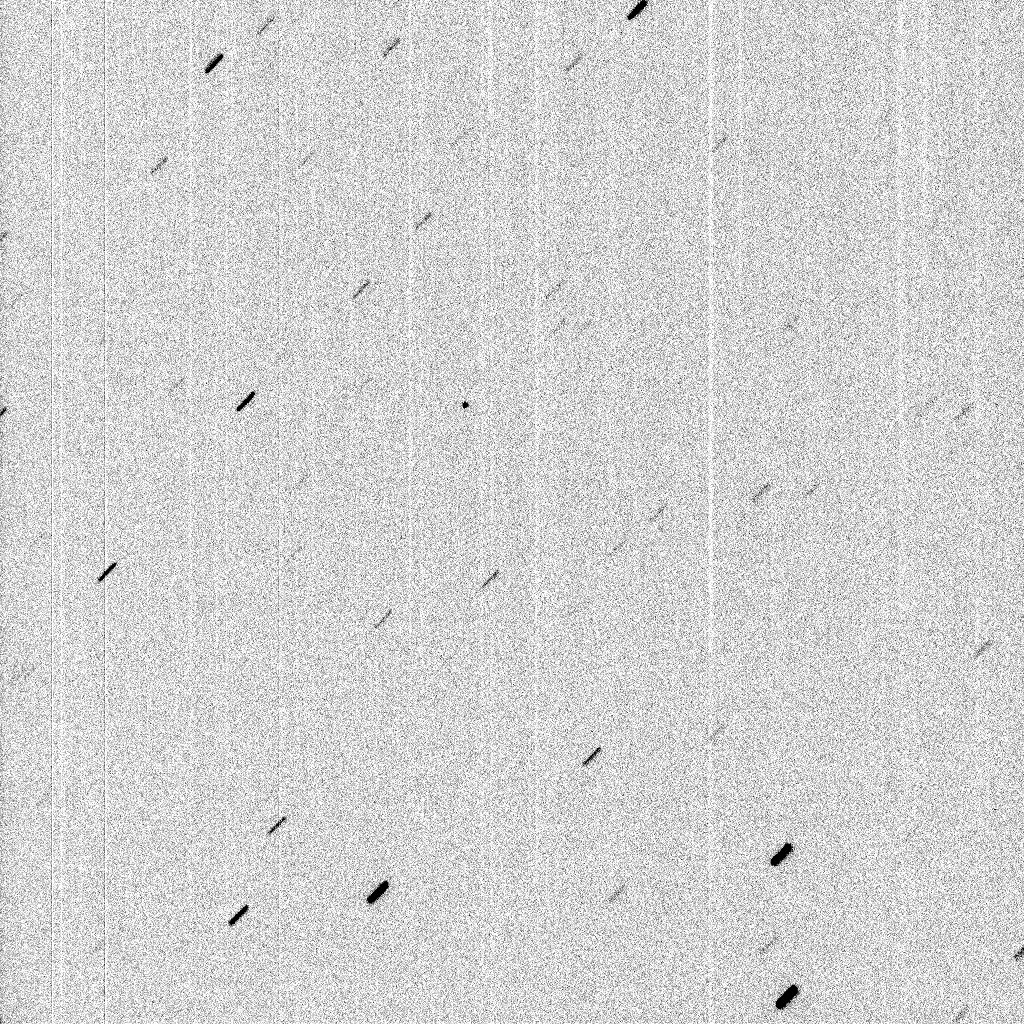
\includegraphics[width=\textwidth]{images/StreakPoint00.jpg}
    \end{subfigure}
    \hfill
    \begin{subfigure}{.3\textwidth}
        \centering
        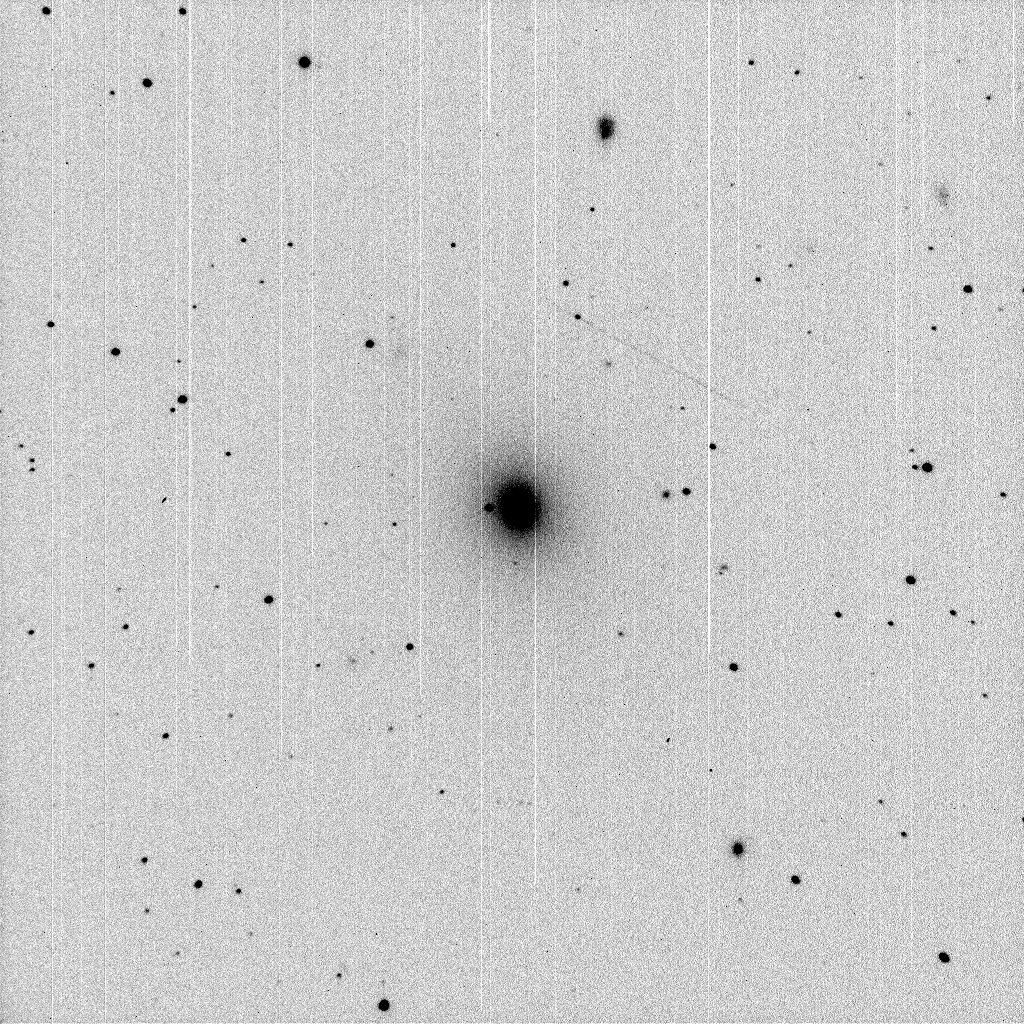
\includegraphics[width=\textwidth]{images/galaxypoints.jpg}
    \end{subfigure}
    \hfill
    \begin{subfigure}{.3\textwidth}
        \centering
        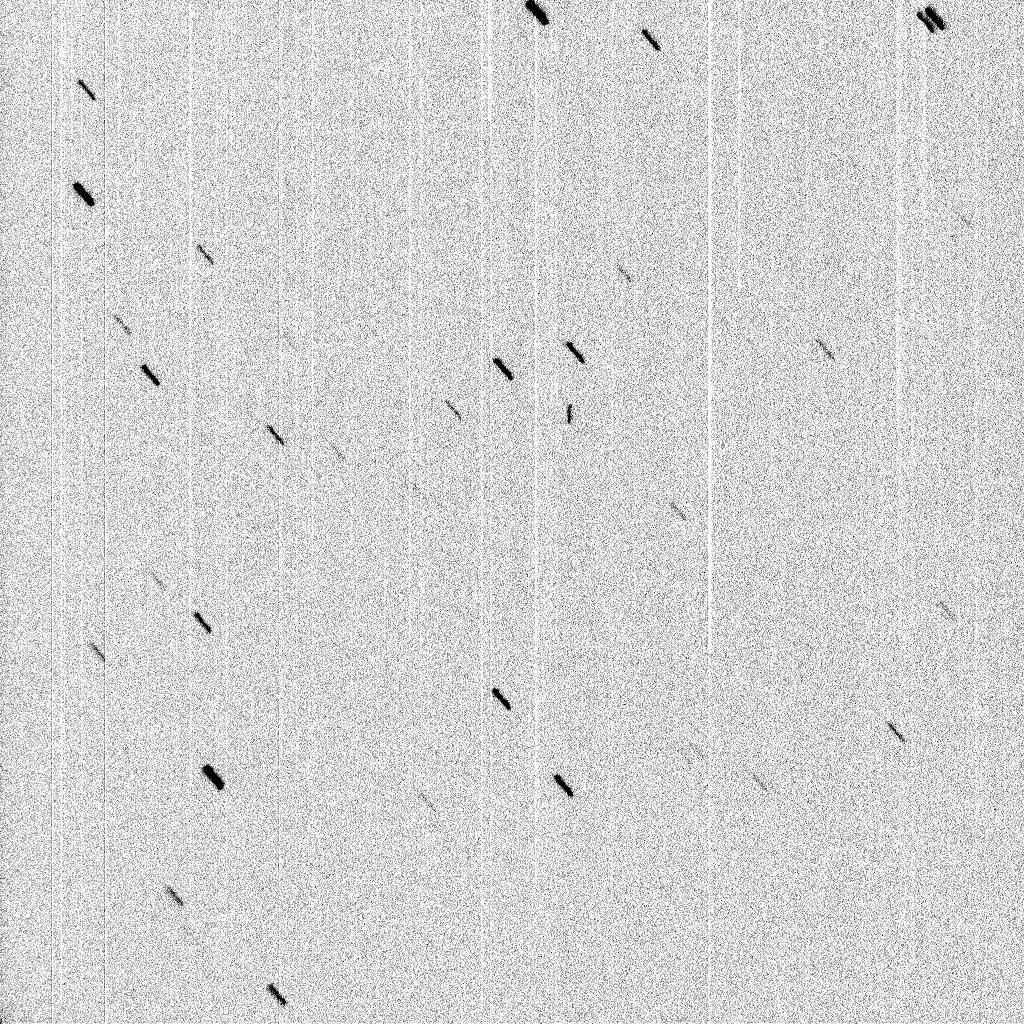
\includegraphics[width=\textwidth]{images/StreakStreak2.jpg}
    \end{subfigure}
    \hfill
    \caption{Examples of some images acquired by AGO70. }
    \label{fig:ago70images}
\end{figure}


%AGO70 has a very thin 700 mm primary parabolic mirror, which is supported by the gravity actuator. The mirror is placed at a focal length of 2962 mm. The telescope is equipped with FLI Proline PL1001 Grade 1 CCD camera and has a 28.5' x 28.5' field of view. Acquired images have a resolution of 1024x1024 pixels and contain values ranging from 0 to 65 535. 

\section{FITS format}
All images acquired from AGO70 are in the format of Flexible Image Transform System (FITS) files. It's an open standard digital format, which is very common for storing astronomical data. This data format will be used within this thesis. The structure of the FITS file is made up of two parts: header and data block \cite{fits}.

A header is a readable data structure that contains multiple keyword/value pairs. It is used for storing image metadata such as size, coordinates, and origin. With astronomical data, the header is very useful in providing photometric and spatial calibration information such as exposure time, readout noise, RADEC coordinates, etc \cite{fits}. An example of the FITS header of the image acquired by AGO70 is shown in the Figure \ref{img:fitsheader}. 

\begin{figure}[h]
    \centering
    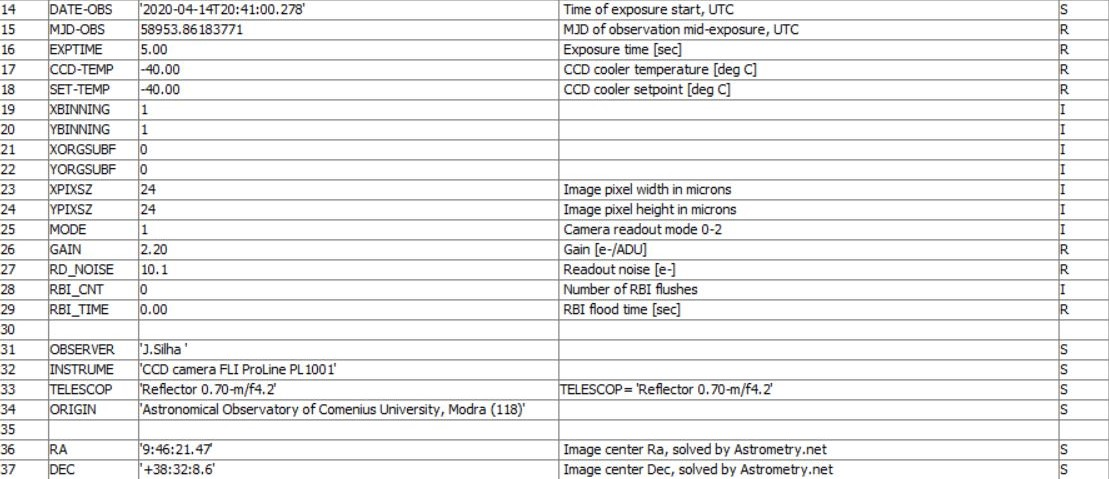
\includegraphics[width=.9\textwidth]{images/fitsheader2.JPG}
    \caption{The FITS header of the image from AGO70.}
    \label{img:fitsheader}
\end{figure}

The data block of the FITS file can store an N-dimensional array of arbitrary size. The data array usually represents an array of image pixel values or tabular data \cite{fits}.
\section{Features} \label{sec:features}
Depending on the relative position and dynamics between the observer
and the object of interest, signals from RSOs can appear differently. The most common shape is a point and streak, which will be explained in greater detail in this section. 

Moreover, other objects like galaxies, nebulas, and comets are present in the universe and can also appear in images. Their profile is significantly different from points and streaks and has more diffuse features. However, for the purpose of this thesis, we will solely focus only on galaxies and more specifically - elliptical galaxies. 
% toto neviem ci tam budem davat lebo tam chcem opisat aj galaxie
%Note, that other types of features exist. Diffuse sources like galaxies or comet tails are less common but cannot be forgotten. However, for this thesis, they are not relevant and we will solely focus only on point-like and streak-like features.   

\subsection{Point}

The shape of the point source of the light on the CCD image is defined by the point spread function - PSF. As the light is passing through the atmosphere, the point on the CCD image is smeared. The smearing effect, also called seeing, is the dominant feature of the PSF. 
Under good optic and tracking conditions, PSF is usually circularly symmetric and can be approximated using a central Gaussian core. The measure used to express the angular size of the PSF is called FWHM - full width at half maximum \cite{romanishin2006introduction}. It measures the diameter of the Gaussian core in half of its maximum amplitude as can be seen in the Figure \ref{img:fwhm0}.  

\begin{figure}[h]
    \centering
    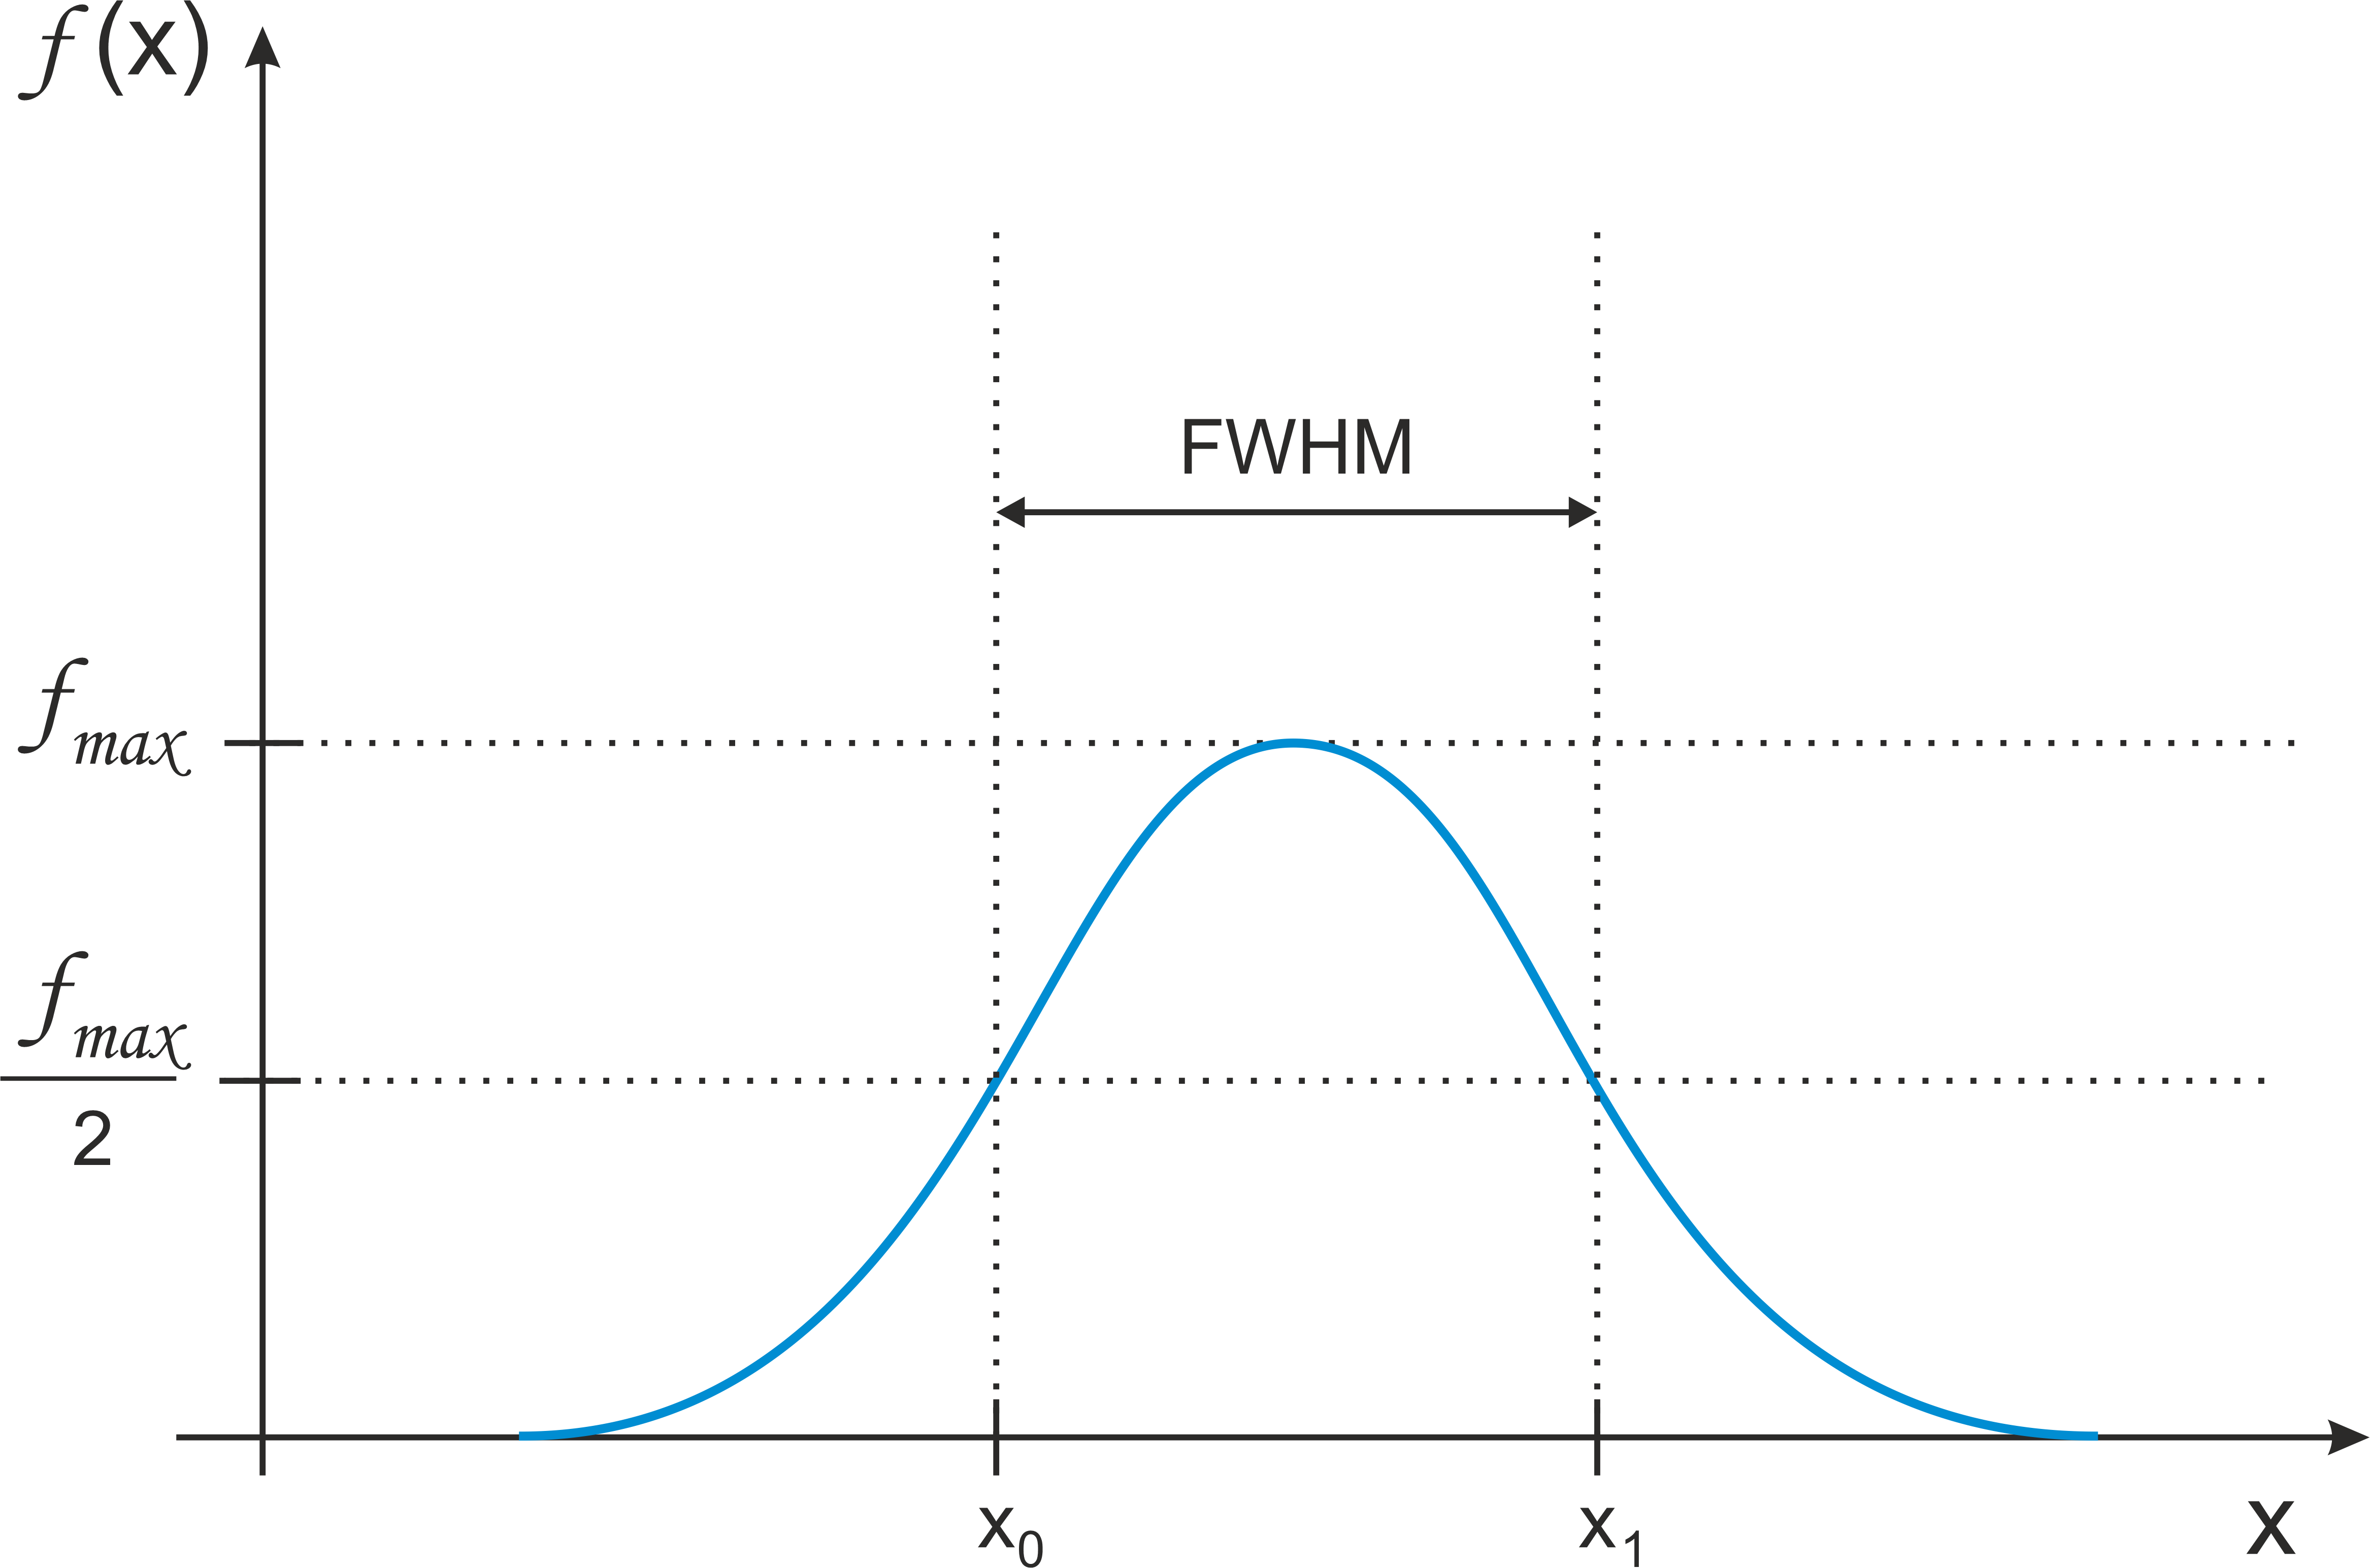
\includegraphics[width=0.5\textwidth]{images/fwhm.png}
    \caption{FWHM shown on the Gaussian curve. }
    \label{img:fwhm0}
\end{figure}

All objects that appear as points on the image, follow the PSF, and therefore all have the same FWHM and shape. However, brighter stars appear bigger on the image and this is caused by the intensity of the pixels belonging to the star \cite{romanishin2006introduction}. This phenomenon is explained in the Figure \ref{img:fwhm01}.


Another important feature of the PSF is that there is no defined edge. The intensity of the function is slowly fading until it blends with the background.


\begin{figure}[H]
    \centering
    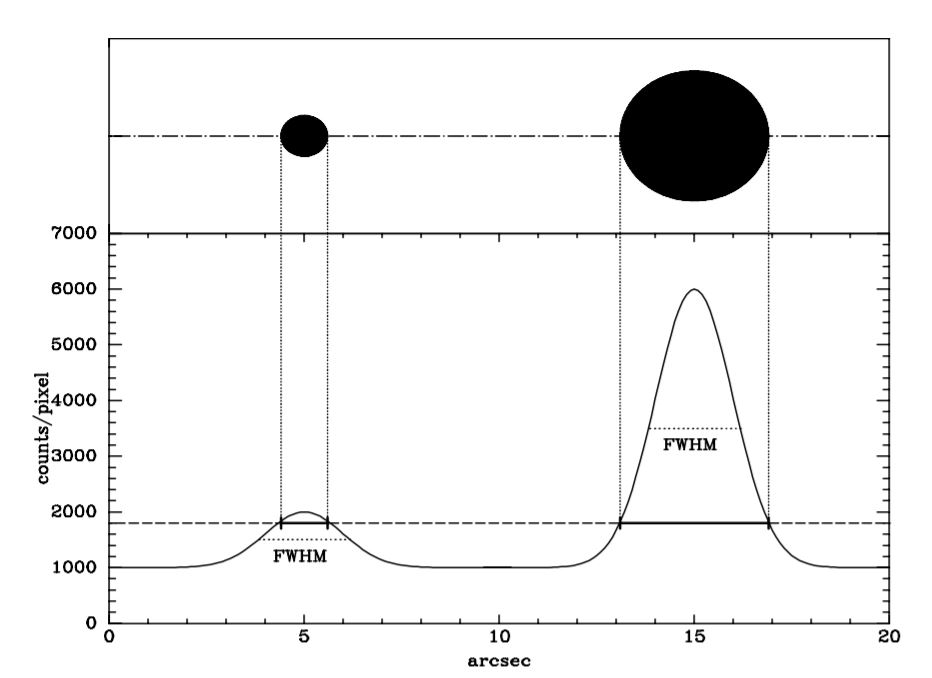
\includegraphics[width=0.7\textwidth]{images/fwhmstars.JPG}
    \caption[Comparison of faint and bright star with the same FWHM and shape]
    {
    The image shows two stars with the same FWHM, but their appearance on the frame (black dots on top of the image) differs significantly. The bright star (right) has flux five times bigger than the faint star (left). 
    On the plot in the bottom part of the image, we can observe the dashed line, which marks 1800 counts/pixel. This means that pixels below, with low intensity, are considered dark, while pixels above are considered brighter or white.  
    First, let's consider a faint star (left) which consists of a few bright pixels, but overall has a very low intensity of pixels. Low-intensity pixels appear black as they are below the dashed line. On the image, the faint star will appear smaller than the brighter star, because only the peak of the PSF will be distinguishable from the dark background. 
    Now consider a bright star (right), which has an overall very high intensity. On the image, the bright star will appear much bigger, because the majority of the PSF is above the dashed line.  
    
    Source: \cite{romanishin2006introduction}.
    
    }
    \label{img:fwhm01}
\end{figure}


\subsection{Streak}

A streak on the image, which resembles a line, can be described by its length, orientation, brightness, and width. 
Streak is approximated using multiple point-spread functions (Gaussian PSFs) moving at a constant rate in one direction and forming a line. PSFs are connected and also overlap each other to form a flat top of the streak-like shape. This function is referred to as PSF-Convolution Trail Function. % citacia

Let's situate a coordinate system on the streak. The direction in which the streak has the highest variance is the $x'$ axis and perpendicular to it is the $y'$ axis. This coordinate system is not consistent with the $(x,y)$ coordinate system of the image. This is because the streak has its orientation $\theta$ and doesn't necessarily need to be aligned with the image coordinate system. 
In this coordinate system, the length of the streak $L$ is measured on the $x'$ axis at the half-height of the function. The projection of the streak signal on the $y'$ axis creates a perpendicular profile of the streak and the width $\sigma$ of the PSF is measured at half-width. This is illustrated in the Figure \ref{img:line0}. 
The flux $f$ of the streak at any point situated in the new orthogonal coordinate system $(x',y')$ can be expressed as:

\begin{equation}
    f(x',y') = b(x',y') + \frac{\Phi}{L} \cdot \frac{1}{\sqrt{2 \pi \sigma^2}} \cdot \int_{-L/2}^{+L/2} 
    exp \left(  
        - \frac{1}{2 \sigma^2} \cdot \left[ (x' - l)^2 + (y')^2 \right]
    \right) \,dl
\end{equation}

where $\Phi$ is the total photometric flux in the streak and $b(x',y')$ is the background flux at the same point \cite{thesisNagy}. 


\begin{figure}[h]
    \centering
    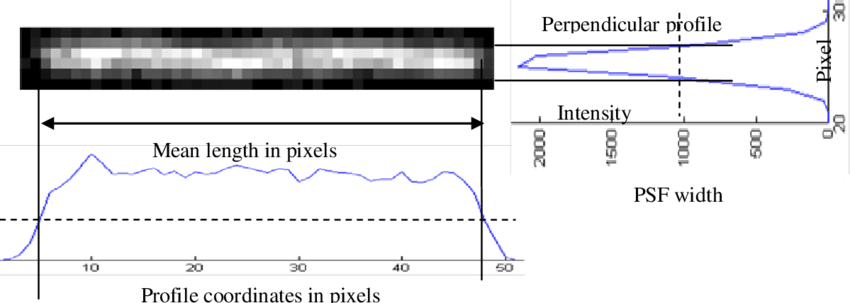
\includegraphics[width=0.7\textwidth]{images/line.png}
    \caption[Length and width of the streak on the image]
    {Length and width of the streak explained on the image.
    Image source: \cite{articleStreaks}.}
    \label{img:line0}
\end{figure}

\subsection{Galaxy}
According to \cite{hubble} galaxies can be classified into 3 categories based on their visual appearance:
\begin{itemize}
    \item Elliptical 
    \item Spiral 
    \item Lenticular
\end{itemize}

In this thesis, we will only focus on the elliptical galaxies, which in the case of modeling and using ellipticity of 1 can also be a good approximation of spiral and lenticular galaxy shapes to be used for the training purposes.

The main characteristic of an elliptical galaxy is that its profile resembles ellipses on the images. They are highly concentrated and the light going from the center fades smoothly and rapidly away. This creates a smooth diffuse profile with an undefined edge. Another interesting feature of elliptical galaxies is that with increasing exposure time of the image, the diameter of the galaxy is steadily increasing but the shape stays roughly the same \cite{hubble}.

Elliptical galaxies are denoted with the letter "E". In full notation "E" is followed by a number representing their degree of ellipticity, which is defined as follows: 

\begin{equation}
E = \frac{(a-b)}{a}
\end{equation}

where $a$ is the major diameter and $b$ is the minor \cite{hubble}. 

\section{Scenarios} \label{sec:scenarios}

In this section, we will explain different scenarios happening during the image capture, that affect how the object appears in the image. Scenarios depend on the mode of tracking (sidereal, object) and the relative velocity between the moving object of interest and the telescope. 

\subsection{Point-like stars, point-like objects}
This is a typical scenario occurring in astronomical images and is shown in the Figure \ref{fig:pointpoint1}. The angular velocity of the moving object of interest is so small that during the exposure time their position on the image doesn't seem to move. The speed is so slow that they don't cross more than one pixel, which leads to the appearance of the object as a point. This applies to both, objects of interest as well as stars. 

This scenario commonly happens in an asteroid field, small solar body system field, and can also appear in space-debris observations when high cadence and low exposure time is used. 

\begin{figure}[!h]
    \centering
    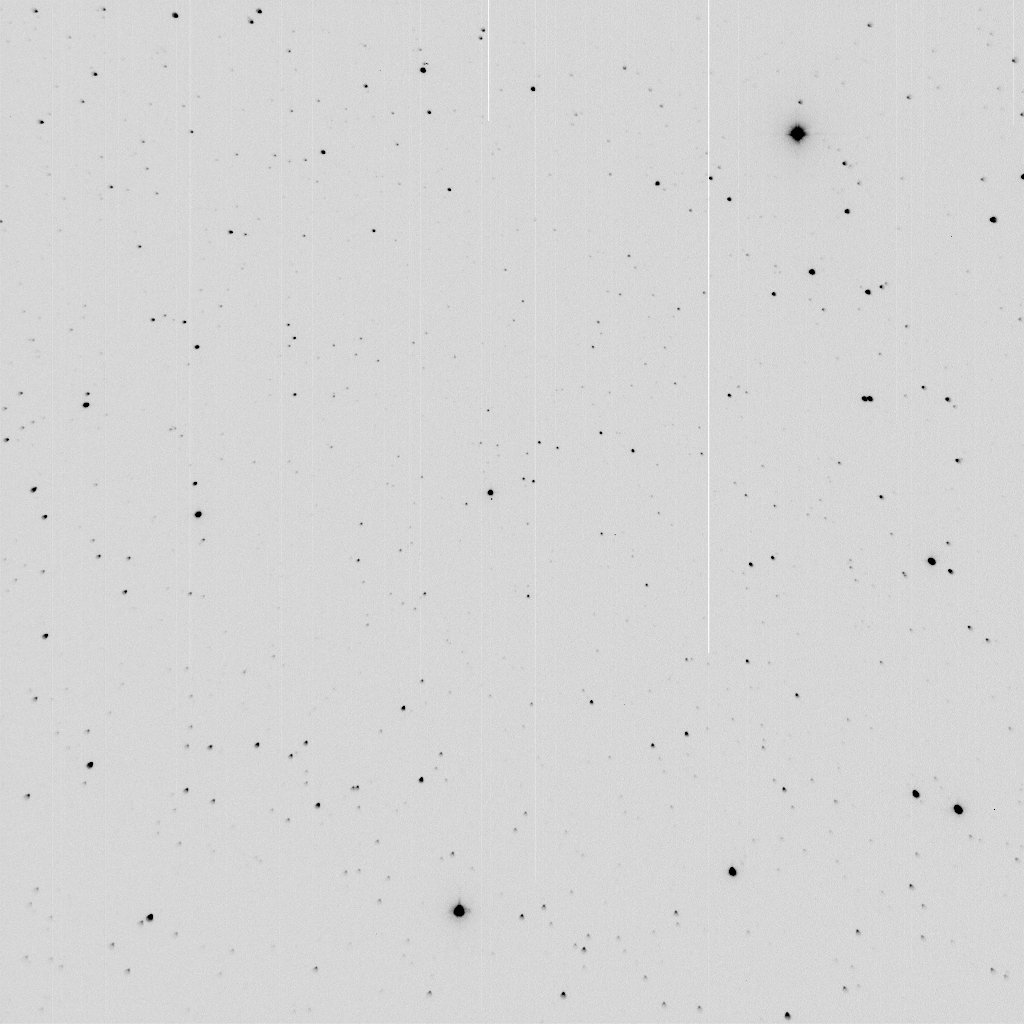
\includegraphics[width=.4\textwidth]{images/PointPoint.png}
    \caption{An example of point-point scenario.}
    \label{fig:pointpoint1}
\end{figure}

\subsection{Point-like stars, streak-like objects}
In ground-based images, stars appear as points, due to slow relative dynamics between the observer. If the exposure time on the image was longer stars would appear as streaks too, as a result of the motion of the Earth. 
During sidereal tracking, the telescope is moving to compensate for the Earth's motion and this results in point-like stars remaining in the same place on images.
In space-based images, stars appear as points if the camera is fixed.


Regarding moving objects, if the exposure time is long enough that the object is crossing more than one pixel, they appear as streaks. This commonly happens when the object is moving with high velocity. %If the exposure time is long compared to the angular velocity, it leads to objects appearing as streaks. 

The point-like stars and streak-like object scenario can be observed in the series of images depicted in the Figure \ref{fig:pointstreak0}.

%However if the exposure time is too short for an object to cross more than one pixel it would appear as a point, which is the point-point scenario explained above. 

\begin{figure}[!h]
    \begin{subfigure}{.3\textwidth}
        \centering
        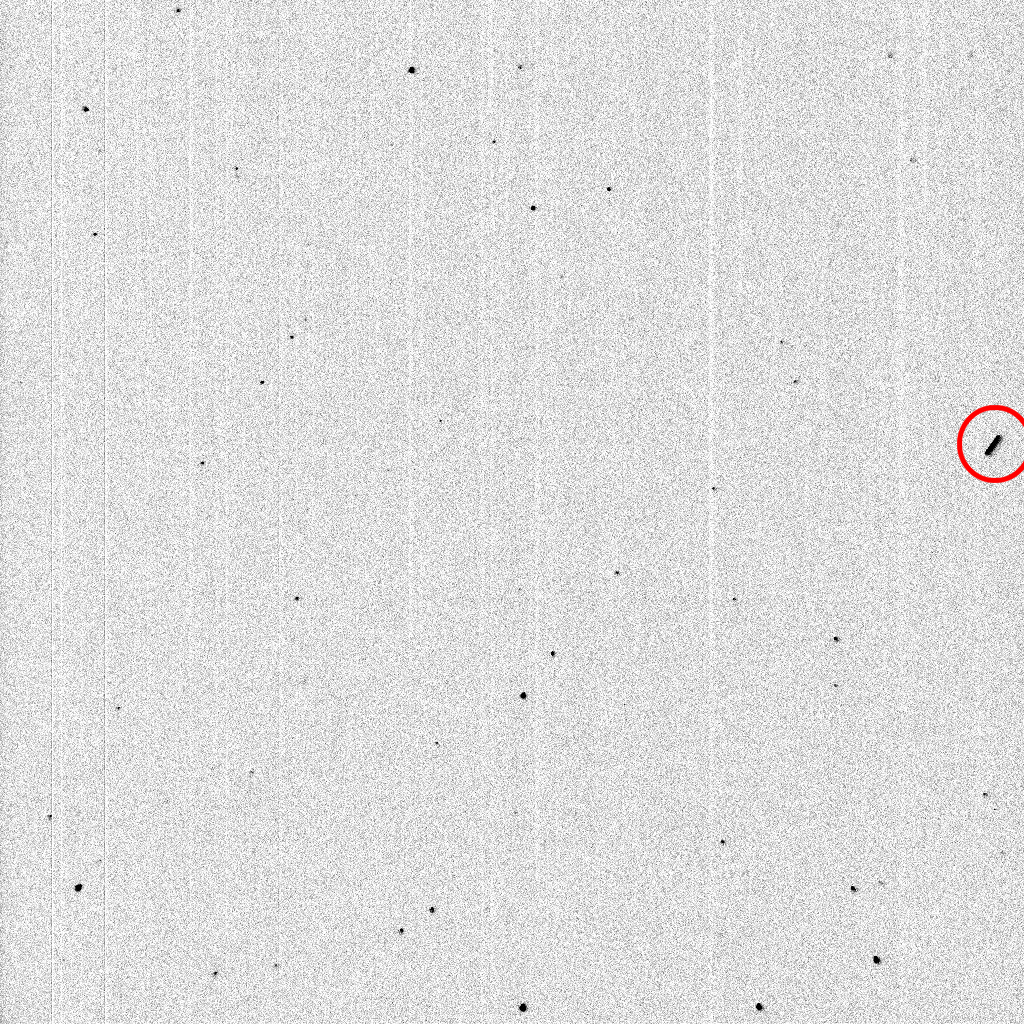
\includegraphics[width=\textwidth]{images/PointStreak1.png}
        \label{fig:pointstreak1}
    \end{subfigure}
    \hfill
    \begin{subfigure}{.3\textwidth}
        \centering
        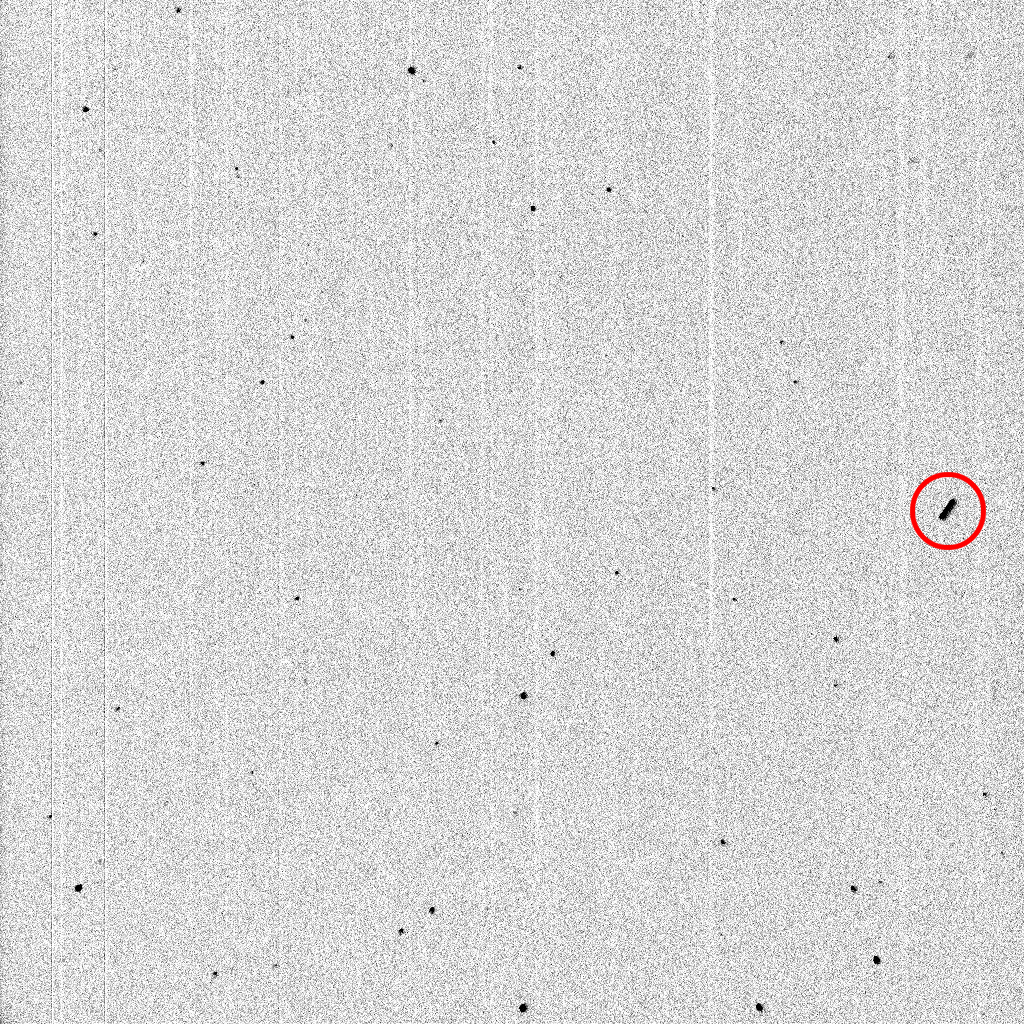
\includegraphics[width=\textwidth]{images/PointStreak2.png}
        \label{fig:pointstreak2}
    \end{subfigure}
    \hfill
    \begin{subfigure}{.3\textwidth}
        \centering
        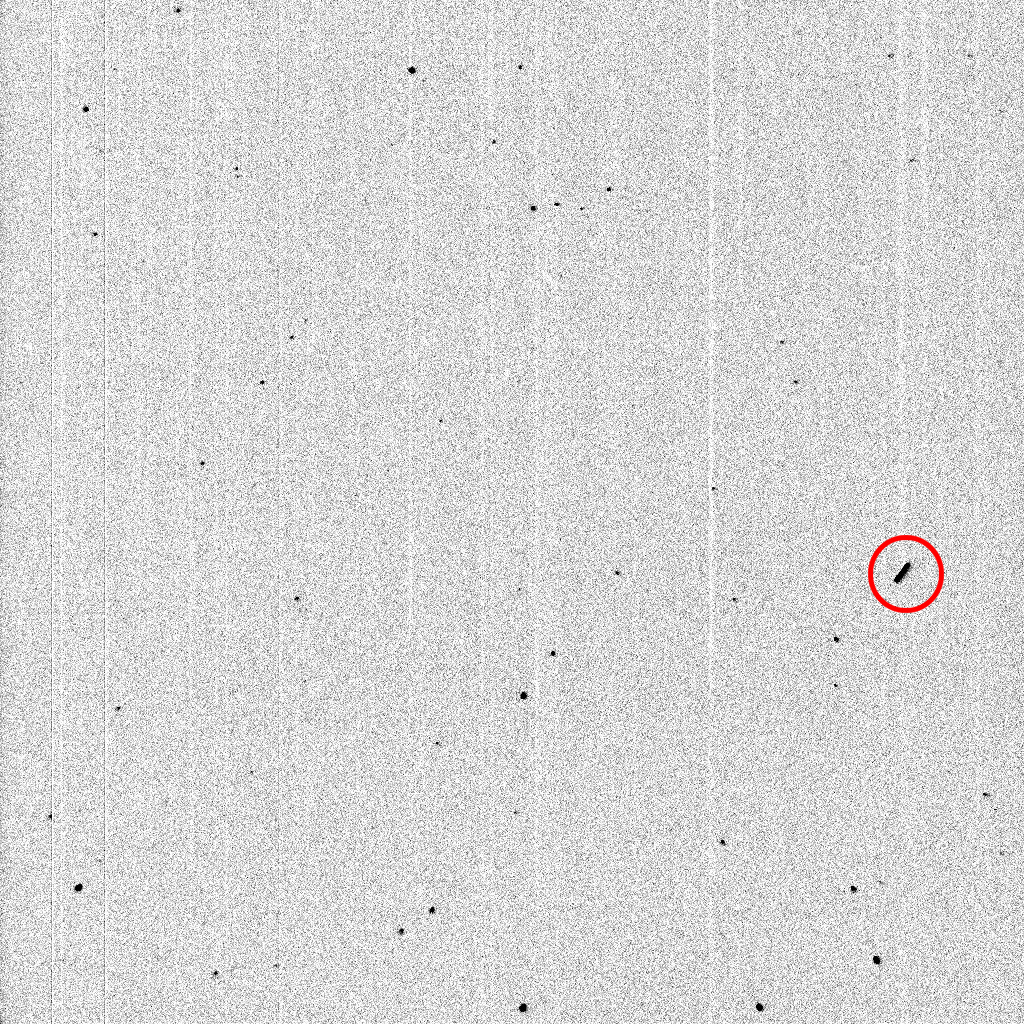
\includegraphics[width=\textwidth]{images/PointStreak3.png}
        \label{fig:pointstreak3}
    \end{subfigure}
    \hfill
    \caption{An example of series of images capturing a streak-like object and point-like stars. }
    \label{fig:pointstreak0}
\end{figure}

\subsection{Streak-like stars, point-like objects}
When the telescope is in object tracking mode, the focus is aimed at the moving object. Thus telescope is following the object matching its speed and direction. The moving object, therefore, appears as a point while stars appear as streaks. All stars will have the same length and direction of the streak-like shape. An example of one point-like object and otherwise streak-like stars are shown in the Figure \ref{fig:streakpoint0}. 

If there are more moving objects present on the frame, they can either appear as points or streaks. In case the other moving objects are moving at a similar speed and direction as the tracked object, they will also appear as points. This scenario happens when a telescope is tracking a cluster of objects. Otherwise, if other objects have different speeds and directions, they will appear as streaks but with different lengths and directions as streaks created by stars. 
This applies to both, space- and ground-based images. All these effects can influence the performance of segmentation or recognition algorithms.

\begin{figure}[!h]
    \begin{subfigure}{.3\textwidth}
        \centering
        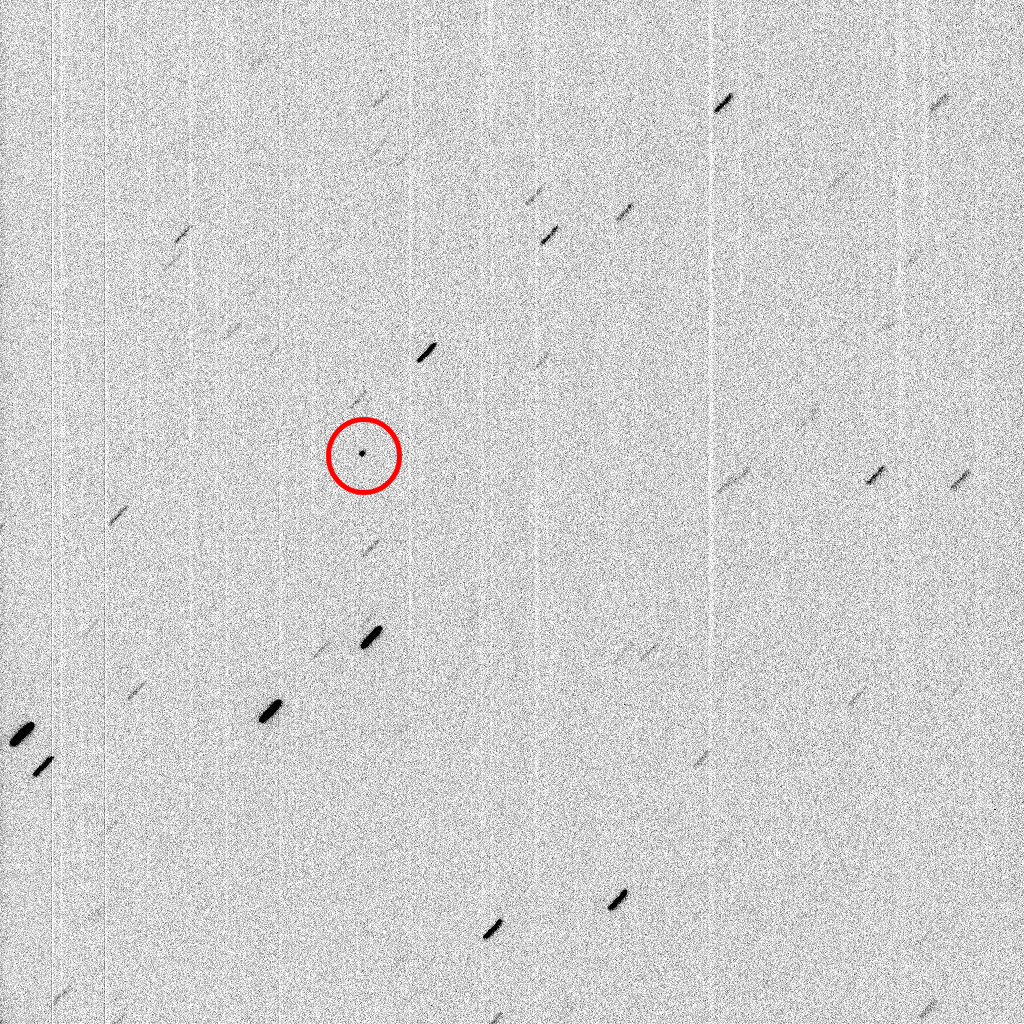
\includegraphics[width=\textwidth]{images/StreakPoint1.png}
        \label{fig:streakpoint1}
    \end{subfigure}
    \hfill
    \begin{subfigure}{.3\textwidth}
        \centering
        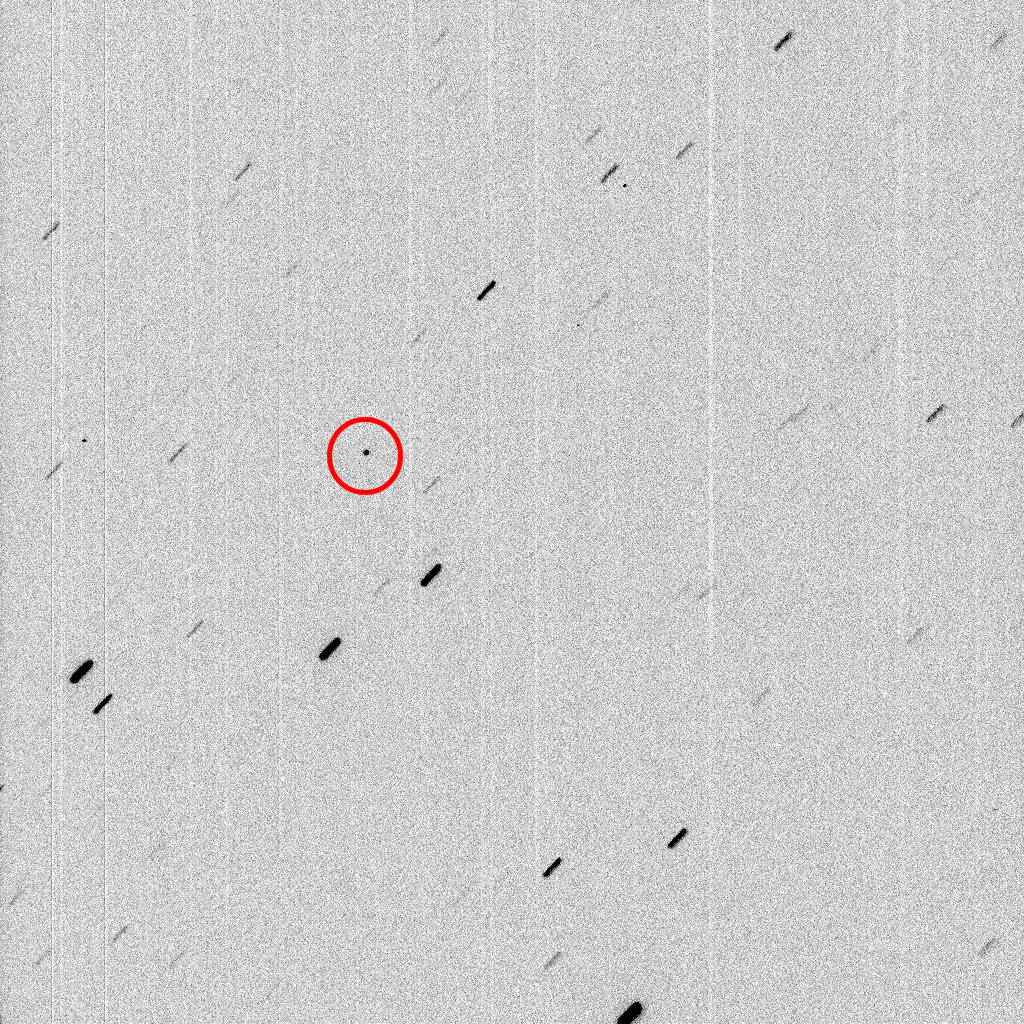
\includegraphics[width=\textwidth]{images/StreakPoint2.png}
        \label{fig:streakpoint2}
    \end{subfigure}
    \hfill
    \begin{subfigure}{.3\textwidth}
        \centering
        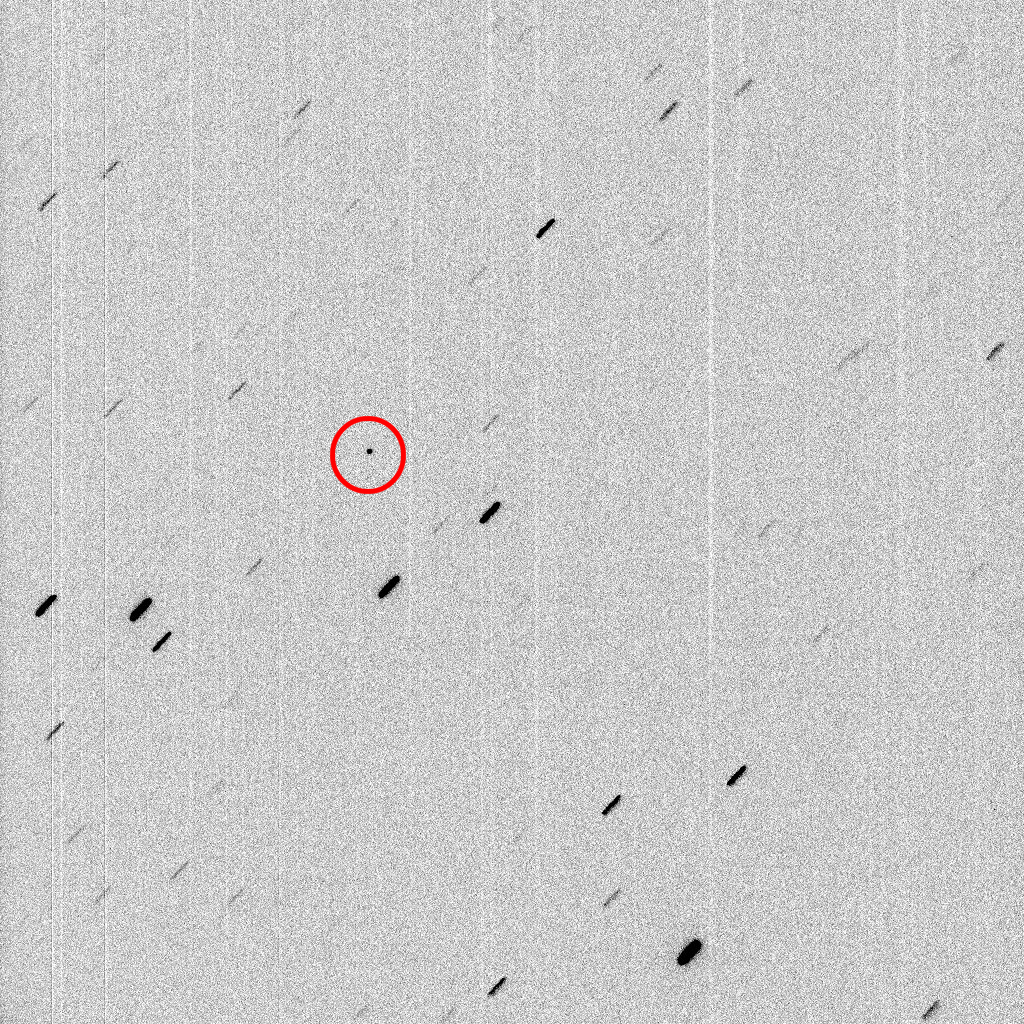
\includegraphics[width=\textwidth]{images/StreakPoint3.png}
        \label{fig:streakpoint3}
    \end{subfigure}
    \hfill
    \caption{An example of series of images capturing a streak-like stars and one point-like object. }
    \label{fig:streakpoint0}
\end{figure}

\subsection{Streak-like stars, streak-like objects}
This is a common scenario happening during the survey of the sky, when stars nor objects are being tracked, which is depicted in the Figure \ref{fig:streakstreak0}. When taking an image of the sky field during the survey, unknown objects can appear randomly, leaving streak-like features of different lengths and directions on the image. 
Stars appear as streaks in ground-based observations due to the motion of Earth and long exposure time. However streak-like stars can also be caused by the motion of the telescope in both ground and space-based observations. 

\begin{figure}[!h]
    \begin{subfigure}{.3\textwidth}
        \centering
        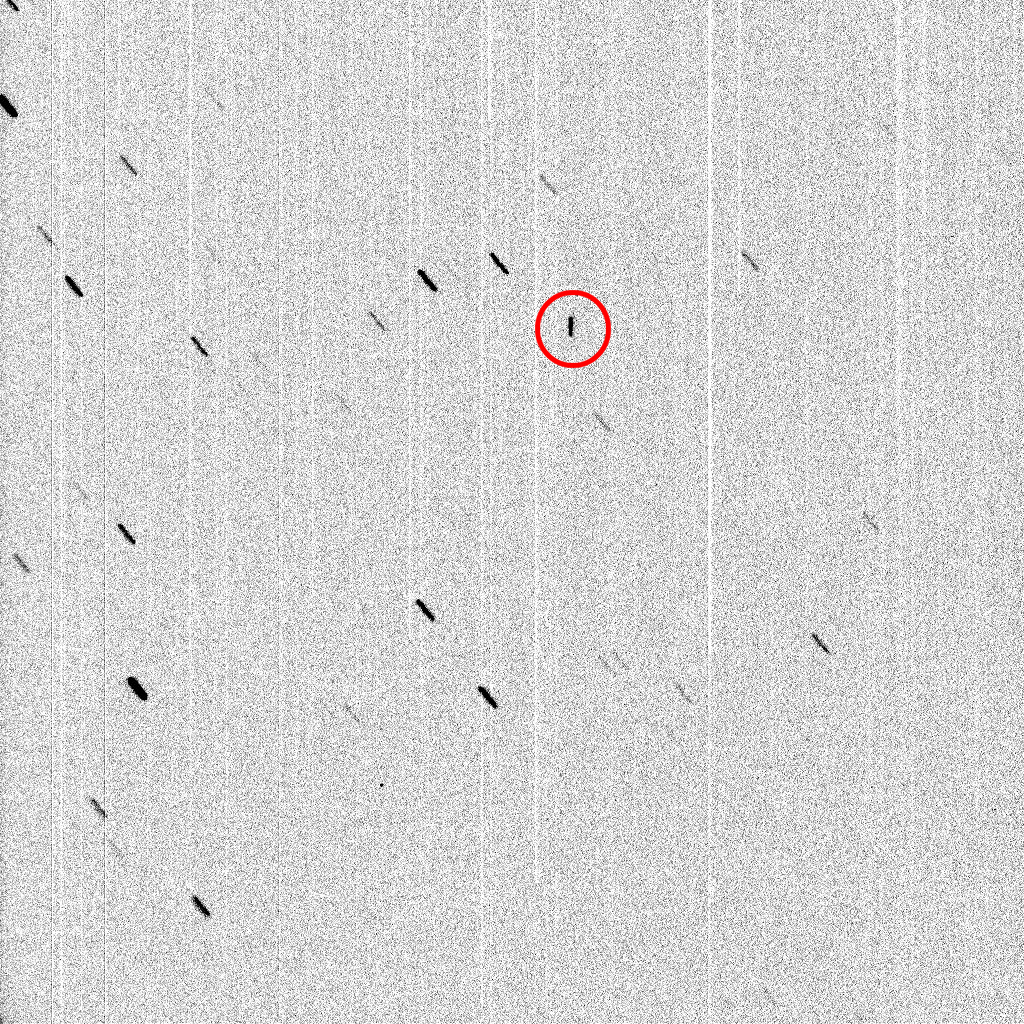
\includegraphics[width=\textwidth]{images/StreakStreak1.png}
        \label{fig:streakstreak1}
    \end{subfigure}
    \hfill
    \begin{subfigure}{.3\textwidth}
        \centering
        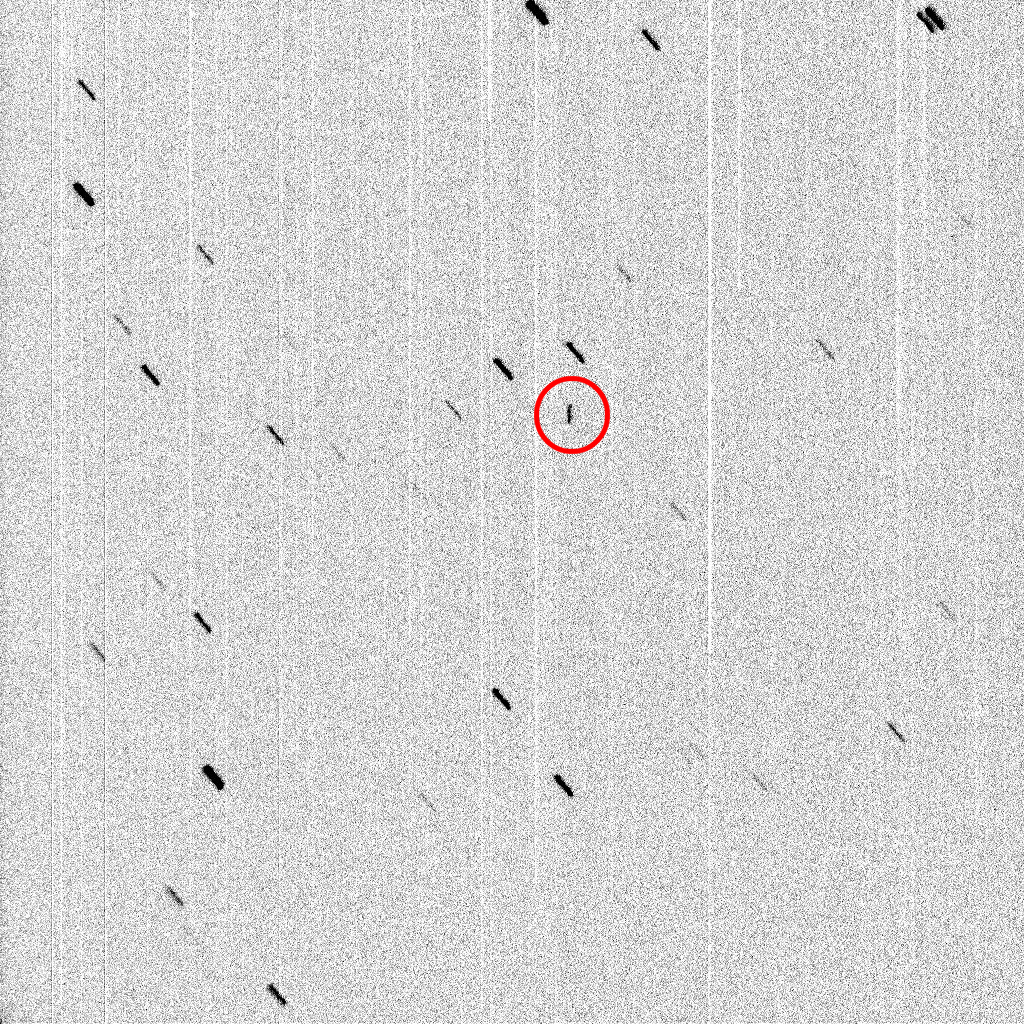
\includegraphics[width=\textwidth]{images/StreakStreak2.png}
        \label{fig:streakstreak2}
    \end{subfigure}
    \hfill
    \begin{subfigure}{.3\textwidth}
        \centering
        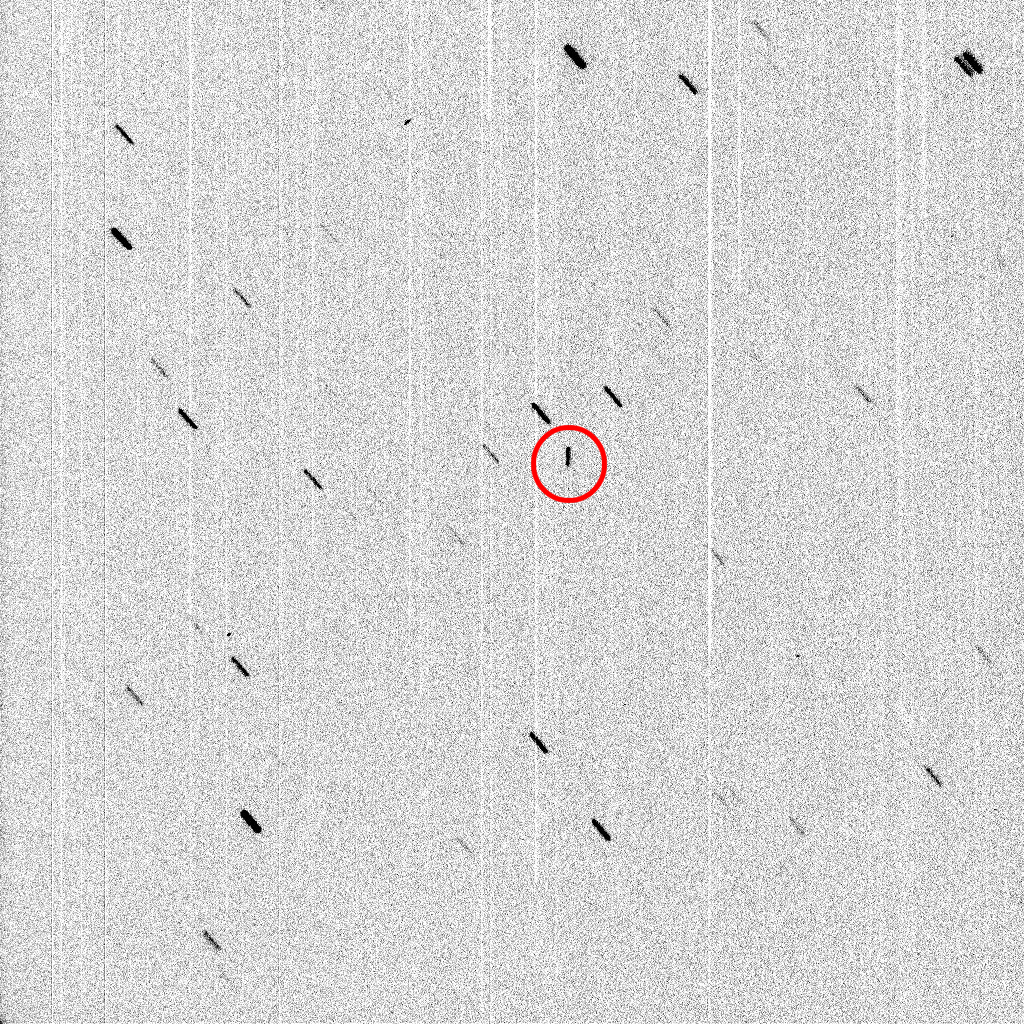
\includegraphics[width=\textwidth]{images/StreakStreak3.png}
        \label{fig:streakstreak3}
    \end{subfigure}
    \hfill
    \caption{An example of series of images capturing a streak-like stars and one streak-like object. }
    \label{fig:streakstreak0}
\end{figure}

\subsection{Supported defects and noises}
To make images realistic, defects and noises that corrupt real astronomical images were added to the generator. 
This includes noises such as Gaussian noise and Poisson noise and defects like hot pixels and cosmic rays. We are aware that some noises and defects are missing. However, the data generator was not the primary focus of the thesis and was only a secondary tool to generate images for training purposes. Yet to make up for missing noises, we added the option to use real BIAS, DARK and FLAT FIELD frames in the generation. These real frames already include readout noise, bias voltage, dark current, dead columns, dust rings, vignette, and others (more info in Section \ref{sec:defects}). 

\subsubsection{Gaussian noise}
Gaussian noise is used to simulate the sky background noise. It is applied to each frame separately to keep the randomness in the images. The user can define the $mean$ and standard deviation ($std$) of the noise.

\subsubsection{Poisson noise}
Poisson noise is applied to each generated object to simulate the photons falling onto the chip. In the configuration file, the user can define if he wants to apply the Poisson noise using the $applyPoisson$ boolean parameter. 

\subsubsection{Hot pixels}
In the generation of hot pixels on the image, the user can set their $count$ and $brightness$. In generated series, hot pixels are static and stay at the same position in all frames. 

\subsubsection{Cosmic rays}
In the configuration file, the user can set the number of generated cosmic rays with $count$, as well as their $brightness$. In Section \ref{sec:defects} we mentioned three different types of cosmic rays: spots, tracks, and worms. Spots usually have fewer pixels than tracks and worms, which is why the user can define the number of pixels using $spotPixelCount$ for spots and $pixelCount$ for tracks and worms. Cosmic rays are generated randomly for each frame since in the real observations they occur randomly as well.

\subsubsection{BIAS, DARK, FLAT FIELD frames}
When using real frames, the user must define the path to the real images using parameter $dataDir$. Important to note, that the images must have the same dimensions as the generated image, or else it will not work correctly. The same real frames are applied to each frame after all objects are generated. First, we multiply the image with the values from the FLAT FIELD frame, which defines the pixel sensitivity. DARK and BIAS frames are added afterward. DARK frames usually already contain bias voltage, so we don't need to apply the BIAS frame.




\section{Photometric reduction of CCD images} \label{sec:photoreduction}


An image obtained by a telescope using a CCD camera is called a raw image. A raw image is affected by before mentioned defects and noises. Therefore, the image needs to be corrected to a certain level to obtain precise photometric results \cite{articleParimucha}. This process is called image calibration, which contains several steps discussed here below.  

\subsection{Calibration images}
The image calibration consists of three steps: subtraction of BIAS image, subtraction of DARK image and division by FLAT FIELD image.

    %%%%%%%%%%%%%%%%%%%%%%%%%%%% 
    \subsubsection{BIAS frame}
    As mentioned earlier, to solve an issue with negative values in ADC, bias voltage was introduced.
    However, during photometry, the offset bias value needs to be subtracted from the image to achieve correct values. To retrieve the bias values on the pixels, the BIAS frame is created. 
    The aim is to retrieve an image without any residual signal in the pixels originating from the camera. This is achieved by taking an image with a closed shutter and zero exposure time \cite{articleParimucha}.
     
             
    %%%%%%%%%%%%%%%%%%%%%%%%%%%%   
    \subsubsection{DARK frame} 

    DARK frames are introduced to detect dark current in the image. Apart from that, they are also capable of detecting hot and dead pixels on the image. 
    To create a DARK frame, an image is taken with a closed shutter to eliminate photo-electrons from stars and the sky. Values in the pixels are from the dark current and bias voltage. Therefore to obtain a correct DARK frame, bias values need to be subtracted from the DARK frame. 
    As mentioned before, dark current is proportional to chip temperature and exposure time. This implies that in order to have correct dark current values, the DARK frame needs to be taken with the same exposure time as the raw image. The same goes for the temperature of the CCD chip \cite{articleParimucha} \cite{articleCcdOnline} \cite{phy217}. 
    

    %%%%%%%%%%%%%%%%%%%%%%%%%%%%  
    \subsubsection{FLAT FIELD frame} 
    
    Taking an image of the perfectly uniform light source, would not result in an image with the same amount of counts in each pixel. Readout noise, bias voltage, and dark current are all contributing to this fact. However, even without them, the image would not be uniform. The main reason is the sensitivity of each pixel. Due to the manufacturing limitations, no two pixels convert the light photons into electrons the same way \cite{articleCCDartifacts} \cite{phy217}.
    
    The solution to this problem is by taking a FLAT FIELD frame, which corrects pixel to pixel sensitivity. As mentioned before, the frame is created by taking a picture of an evenly illuminated field. One of the most common ways is to take an image of the twilight sky.
    Similarly, as with the DARK frame, this FLAT FIELD frame contains values from bias voltage as well as dark current. To get a single correct FLAT FIELD frame, these values need to be subtracted.
    Another great feature of the FLAT FIELD frame is that it can also detect dust particles on the filters and lenses. These manifest as dark rings on the image. They are the same with different exposure times but vary from filter to filter. However, they also differ from time to time as some particles can be shifted, eliminated, or added. 
    Furthermore, flat fielding can clear dimming on the edge of the image. This is also called vignetting and is caused by out-of-focus obstructions in the light path \cite{articleParimucha} \cite{phy217}.
    
    After taking the FLAT FIELD frame, signal values are arbitrary, since it only means how bright the source of illumination was. The important part is the differences in the signal across the chip. FLAT FIELD frame is therefore normalized in a way that the average signal in each pixel is 1 \cite{phy217}.
    %% najst citaciu tohto
    
        
    %%%%%%%%%%%%%%%%%%%%%%%%%%%%  
    \subsubsection{MASTER frame}
    
    Due to the nature of reading the image from the CCD chip, every calibration image contains readout noise, which can cause issues during the calibration process. To minimize the noise, multiple calibration images are taken, which are then reduced to one MASTER frame. 
    The MASTER frame is created by taking average or median values of the pixel from the multiple calibration images (BIAS, DARK, FLAT FIELD).
    After the process, we have MASTER BIAS, MASTER DARK, and MASTER FLAT FIELD frames (shown in the Figure \ref{fig:masterframes}), and these are later used in photometric reduction \cite{articleParimucha}.
   
   
   
    \begin{figure}[!h]
    \centering
        \begin{subfigure}[t]{.3\textwidth}
            \centering
            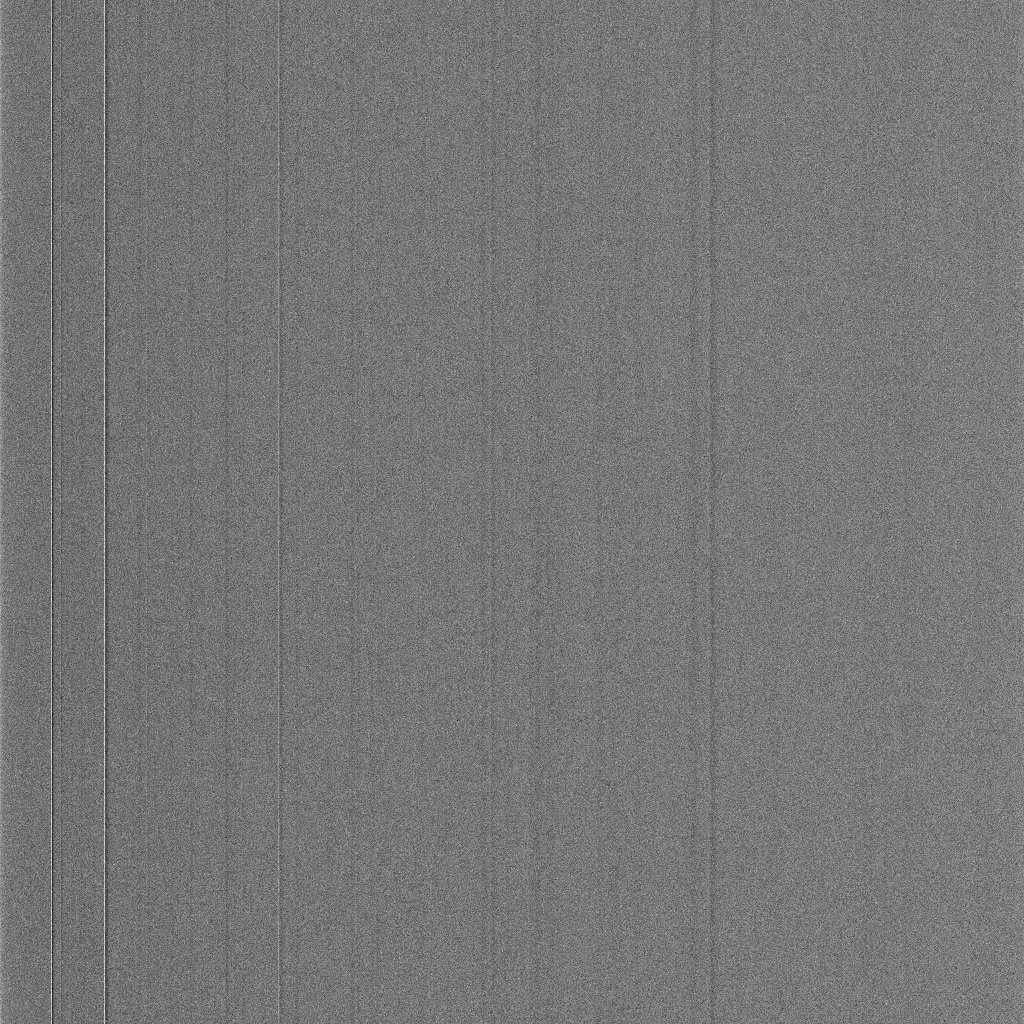
\includegraphics[width=\textwidth]{images/biasframe.jpg}
            \caption{MASTER BIAS frame.}
            \label{fig:biasframe}
        \end{subfigure}
        \hfill
        \begin{subfigure}[t]{.3\textwidth}
            \centering
            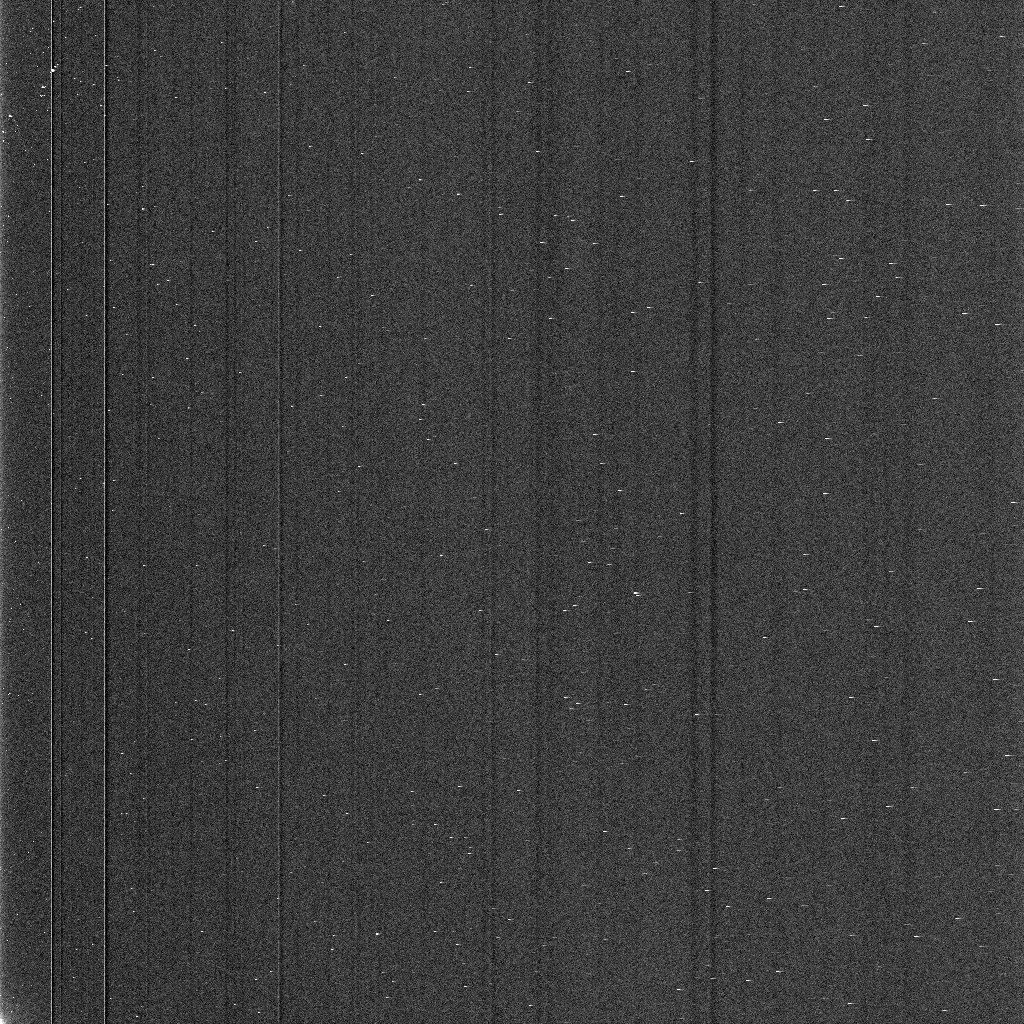
\includegraphics[width=\textwidth]{images/dark90s.jpg}
            \caption{MASTER DARK frame with exposition time of 90 seconds.}
            \label{fig:darkframe}
        \end{subfigure}
        \hfill
        \begin{subfigure}[t]{.3\textwidth}
            \centering
            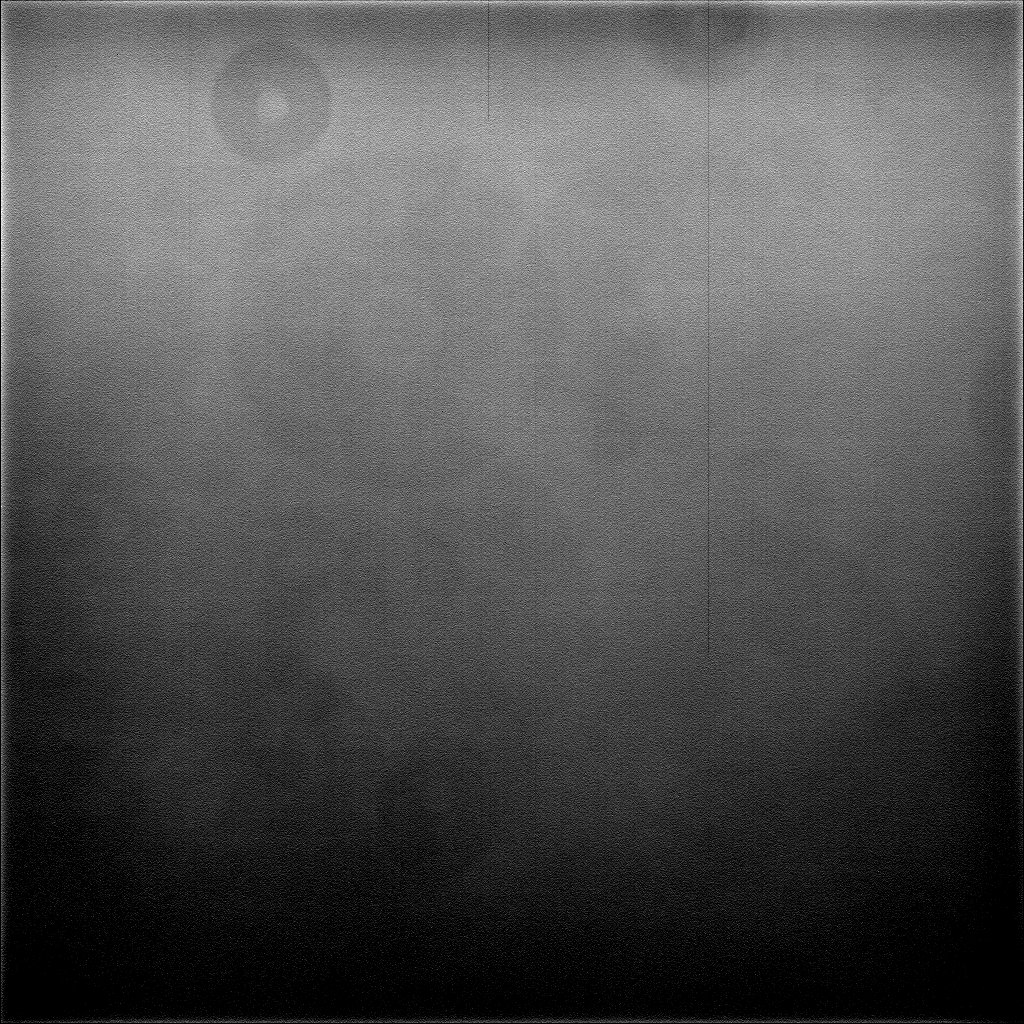
\includegraphics[width=\textwidth]{images/flatframe.jpg}
            \caption{MASTER FLAT FIELD frame.}
            \label{fig:flatframe}
        \end{subfigure}
        \hfill
        \caption{Examples of MASTER frames acquired by AGO in Modra.}
        \label{fig:masterframes}
    \end{figure}



\subsection{Formal definition}

The intensity of the raw image at the pixel $(x,y)$, with exposure time $t$ and temperature of CCD chip $T$ can be generally written as
\[ I(x,y,t,T) = b(x,y,T) + d(x,y,t,T) + i(x,y,t,T) f(x,y,t_f,T) \]

where $b(x,y,T)$ is the intensity of BIAS frame. Exposure time is ommited since the BIAS frame is taken with exposure time of zero. Intensity of DARK frame is denoted as $d(x,y,t,T)$. $f(x,y,t_f,T)$ is the response factor of FLAT FIELD frame, taken with exposure time $t_f$ \cite{articleParimucha}.

The intensity of the real object, which we want to obtain is denoted as $i(x,y,t,T)$. 
All the images are dependent on temperature $T$, which can be omitted from the equation since the CCD chip is cooled down and images are usually taken with the same temperature \cite{articleParimucha}.

To get the real intensity of the object the previous equation becomes
\[
i(x,y,t) = \frac{ I(x,y,t) - b(x,y) - d(x,y,t)}{f(x,y,t_f)}
\]

